%!TEX root = thesis.tex

\chapter{Implementation}

My largest contribution to the project of component-based garbled circuits is the implementation of the theoretical ideas in a program called \CompGC. 
The aim of \CompGC is to run a two party garbled circuit protocol from start to finish. 
The garbler and evaluator simply select a function to compute, plug their inputs into the system, and \CompGC securely computes the function.
This chapter describes the creation of \CompGC and presents experimental results. 

\section{\CompGC}

\CompGC was constructed over the period of 5 months in the programming language C. 
It consists of approximately $5,000$ lines of code, includes a submodule, \LibGarble, and includes python scripts to generate auxiliary files. 

\CompGC started with \JustGarble as its basic building block.
\JustGarble is a C-library written by Bellare et al. \cite{justgarble} that creates a garbled circuit given an inputted circuit, and evaluates the garbled circuit given input labels. 
It is a tool, supporting only garbling and evaluating operations, but does not perform the many operations needed for a whole secure system, like networking, oblivious transfer, and secure recovery of final outputs. 

I later replaced \JustGarble with \LibGarble, an improvement of \JustGarble, which was implemented by my colleague Alex Malozemoff.
\LibGarble made a number of improvements to \JustGarble, including cleaning up the API and improving the memory layout of  data-structures.
These improvements contributed to a substantial increase in performance: evaluating AES uses 17 cycles per gate in \LibGarble versus 22 cycles per gate in \JustGarble, a 22\% improvement. 
\LibGarble also adds the newest cryptographic technique, half-gates; However, \CompGC does not use half-gates since half-gates reduces the size of the garbled table at the cost of a single call to the hash function during evaluation. 
In the component-based garbled circuit setting, the garbled tables are communicated during offline time, and we are most concerned with online time when the hash function would be called; hence half-gates actually reduce performance.

\CompGC has an offline and an online phase. 
In the offline phase, \CompGC takes as input a list of circuits and creates a specified number of each circuit. 
The list of circuits could be small and focused, designed for computing a single function such as AES, or the list could be diverse, allowing for the computation of a variety of functions. 
\CompGC garbles the list of circuits the specified number of times, and then sends the garbled circuits with an attached identification number from the garbler to the evaluator. 
The garbler and evaluator each save the garbled circuits to disk. 
Finally, the garbler and evaluator perform the offline phase of preprocessed oblivious transfer. 
\CompGC uses the Naor-Pinkas semi-honest oblivious transfer protocol; the library for performing oblivious transfer was given to me by Alex Malozemoff \cite{naor-pinkas-ot}. 
The garbler finishes by saving the input labels and oblivious transfer data to disk, and similarly, the garbler saves the oblivious transfer data to disk. 
Algorithms \ref{alg:garbler-offline} and \ref{alg:evaluator-offline} show the steps taken by each party in the offline phase. 

In the online phase, the evaluator begins by loading the function to be computed from disk. 
We specify the function in a JSON format, in which the following information is laid out: components needed in the function, how components input and output wires are linked, where inputs should go, and what wires are outputs. 
We chose to use JSON because the file format is human readable, but a different format, such as a binary format, would be faster. 
As the functions become more complex, it becomes harder to write the function specification files. 
To overcome this, I wrote a python script that automatically generates the function specification file for various functions on arbitrary inputs. 

After the garbler loads the function specification file from disk, it generates a set of instructions for the evaluator. 
The instructions specify what components are used by naming them with the unique identification number assigned in the offline phase. 
The instructions further specify in what order to evaluate components, and how to link components. 
This step requires specifying the output wires of one garbled circuit, the input wires of another garbled circuit, and the linking value.
Finally, the instructions specify how to map the final output wire labels to bits; this works by sending unary gates, with a two-row garbled table, for each output wire. 

After the garbler sends the instructions to the evaluator, they both perform the online phase of oblivious transfer, whereby the evaluator acquires their input labels. 
The garbler next sends the input labels corresponding to their inputs. 
At this point, the evaluator has all the data they need to finish the protocol. 
They follow the instructions, and acquire the output bits. 
Algorithms \ref{alg:garbler-online} and \ref{alg:evaluator-online} summarize the online phase. 

\begin{algorithm}
    \caption{Garbler Offline}
    \label{alg:garbler-offline}
    \begin{algorithmic}
        \State \textbf{Input:} List of circuits, and number of ciphertexts to be OT-preprocessed.
        \State 1. Build circuits
        \State 2. Garble circuits (using \LibGarble)
        \State 3. Assign each garbled circuit an ID
        \State 4. Send garbled circuits and their IDs to evaluator
        \State 5. Save input labels and output labels of garbled circuit to disk
        \State 6. Perform offline phase of OT-preprocessing
        \State 7. Save data from OT-preprocessing to disk
    \end{algorithmic}
\end{algorithm}

\begin{algorithm}
    \caption{Evaluator Offline}
    \label{alg:evaluator-offline}
    \begin{algorithmic}
        \State 1. Receive garbled circuits from garbler
        \State 2. Save garbled circuits to disk
        \State 3. Perform offline phase of OT-preprocessing
        \State 4. Save OT-preprocessing data to disk
    \end{algorithmic}
\end{algorithm}

\begin{algorithm}
    \caption{Garbler Online}
    \label{alg:garbler-online}
    \begin{algorithmic}
        \State 1. Load input labels and output labels of garbled circuits from disk
        \State 2. Load OT-preprocessing data from disk
        \State 3. Load function specification from disk
        \State 4. Generate instructions from function specification
        \State 5. Compute chaining values, and add values to instructions
        \State 7. Perform online stage of OT-preprocessing
        \State 8. Send input wires correspond to garbler's input
        \State 9. Send instructions
    \end{algorithmic}
\end{algorithm}

\begin{algorithm}
    \caption{Evaluator Online}
    \label{alg:evaluator-online}
    \begin{algorithmic}
        \State 1. Load garbled circuits from disk
        \State 2. Load OT-preprocessing data from disk
        \State 3. Perform online stage of oblivious transfer - acquire evaluator's input labels
        \State 4. Receive garbler's input labels
        \State 5. Receive instructions
        \State 6. Following instructions, chaining and evaluating as instructed
    \end{algorithmic}
\end{algorithm}

\section{Experiments}
\CompGC experiments were run on an Intel Core i5-4210H CPU. 
They were conducted over two network settings. 
The first network setting ran both parties on the default localhost configuration, which was measured to have a latency of 0.012 ms and bandwidth of 25.2 Gb per second. 
The second network setting used the built in Linux network emulator {\sf netem} to configure localhost to mimic the latency and bandwidth of the internet. 
This included setting latency to 33 ms and bandwidth to 50 Mbits per second. 
Finally, \CompGC requires reading from disk; our experimental machine was measured to have cache reads speed of 6.7 GB per second and buffered disk reads speed of 96 MB per second.

We ran four experiments: AES, CBC mode, and Levenshtein distance with 30 symbols and with 60 symbols. 

In the AES experiment, we treated each round of AES as a separate component. AES has 10 rounds, and hence required linking 10 components. Moreover, we used 128-bit AES, meaning that each component link required linking 128 wires. 

CBC mode is an algorithm for encrypting messages of arbitrary length using a blockcipher, for which we used AES-128. 
We again used a single round of AES as a component, and we also used XOR component, which took 256 bits of input, and outputted their xor. 
For our experiment, we ran CBC mode on a 10 block message, a 1,280 bit string, thus requiring 110 components - 100 AES round components and 10 XOR components. 

Levenshtein distance is a measure of the difference between two strings which counts the minimum number of insertions, deletions or substitutions needed to transform one inputted string into the other inputted string. 
The most popular algorithm for computing Levenshtein distance is a dynamic program that runs in $\Theta(n^2)$. 
The algorithm is  two nested for loops where we run a procedure called \textit{Levenshtein-core} inside the inner for loop. 
Levenshtein-core takes five inputs - three distance values and two symbols - and it computes a new distance based on those five values.
For more information on the Levenshtein distance algorithm, we refer the reader to \cite{wiki-leven}. 

For our Levenshtein experiment, we use the Levenshtein-core circuit as a our only component; see figure \ref{fig:leven-core} for a description of the component.
If Levenshtein is being run on $n$-bit inputs, then we use $n^2$ Levenshtein-core components. 
Our experiment used an 8-bit alphabet and ran Levenshtein distance on strings of length 30 symbols and on strings of length 60 symbols, corresponding to 900 and 3600 components respectively. 

\begin{figure}
    \center
    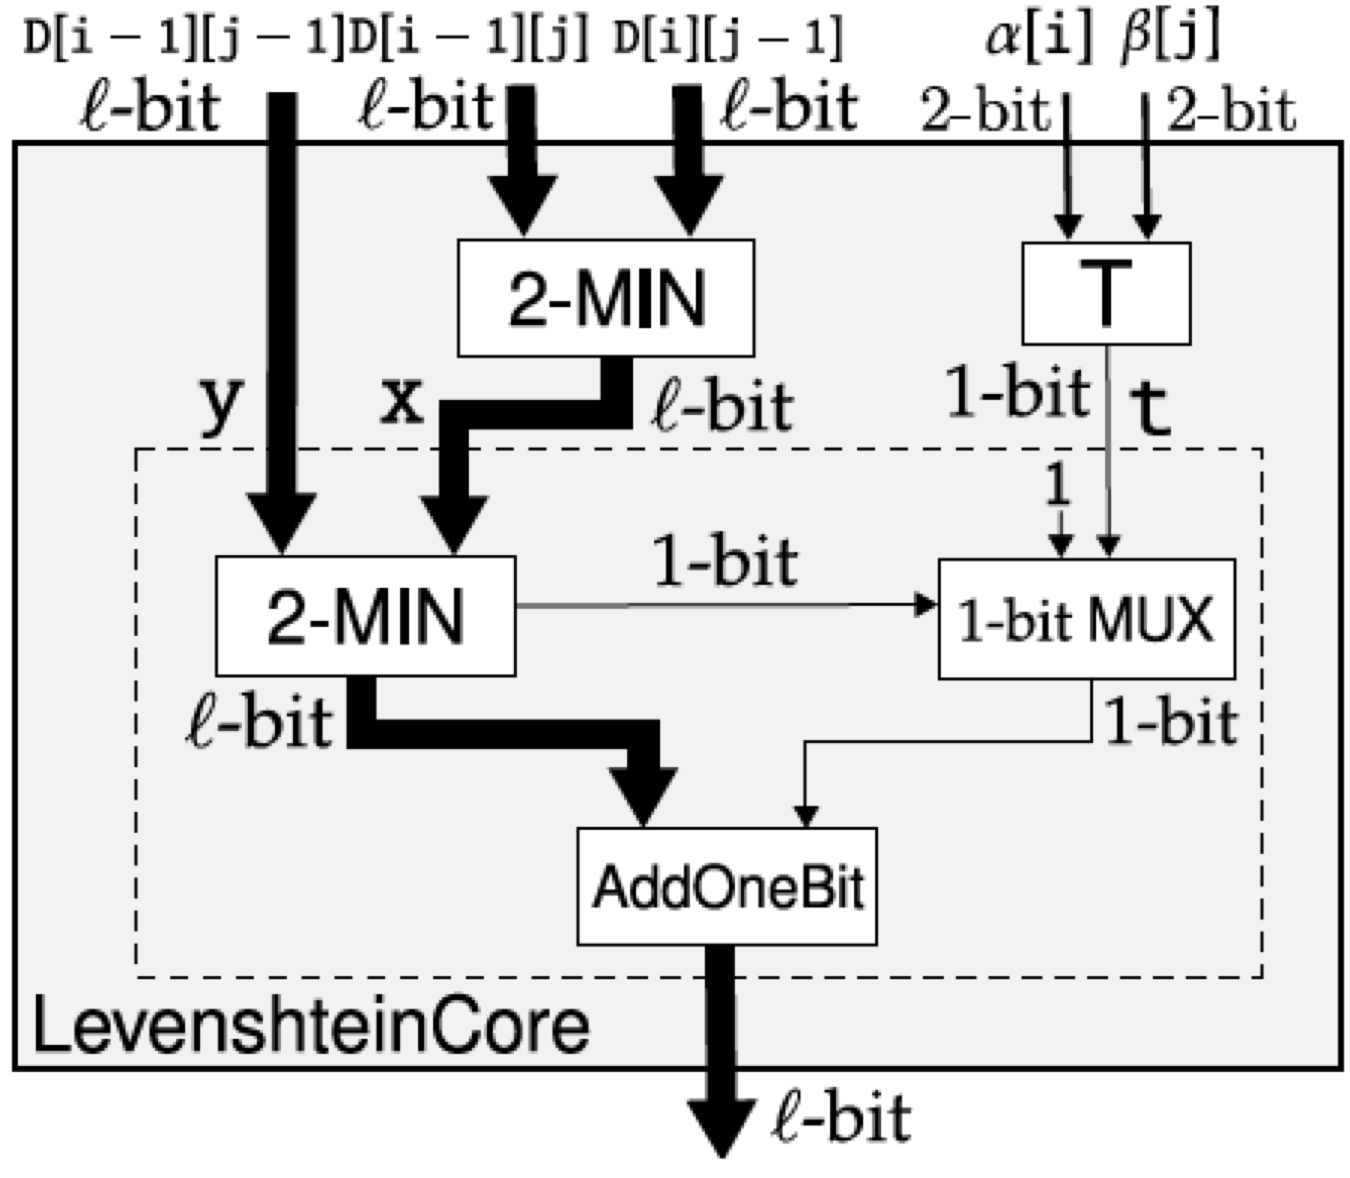
\includegraphics[scale=0.3]{images/leven_core}
    \caption[Levenshtein-core component]{The Levenshtein-core component used in the Levenshtein distance algorithm. 
    Levenshtein distance is a dynamic algorithm, and this is the only component used. 
    This particular version of Levenshtein-core was designed by \cite{faster2pc}.}
    \label{fig:leven-core}
\end{figure}

\section{Results}

\al{Should I say that I didn't run the experiments? That seems relevant.}

We ran experiments on the \CompGC system to compare component-based garbled circuits to standard 2PC garbled circuits, and to compare standard component-based garbled circuits to SCMC.

Table \ref{tbl:results} shows the online evaluator computation time, including time to load data from disk, of standard 2PC garbled circuits (implemented inside of the \CompGC system) and component-based garbled circuits with SCMC.
We give the average time of 100 trials and the 95\% confidence interval, the value after the $\pm$.
We see that larger circuits - Levenshtein 60 - offer more time savings than smaller circuits - AES; this is expected, since standard garbled circuits require that the entire circuit is communicated during online time, whereas the component-based garbled circuits sends the circuit during the offline phase. 

Table \ref{tbl:results-no-load} shows the same timing as table \ref{tbl:results} except we remove the time spent loading from disk.
Since \CompGC employs an offline phase, data is loaded from disk in the online phase. 
Table \ref{tbl:results-no-load} can be misleading - in what application do we assume that data is preloaded into RAM?
We include table \ref{tbl:results-no-load} because the literature often reports these times \cite{blazing-fast}. 
The times do have merit, as they highlight how CPU-bound the computation is, as opposed to measuring reading-from-disk speed, which can vary widely and is not something over which algorithm creators or programmers have much control. 

Table \ref{tbl:results-scmc} compares the speed of standard component based garbled circuits to SCMC.
We see approximately a 2x improvement for all of the experiments. 
However, these experiments do not highlight the benefit of SCMC. 
SCMC offers the greatest benefits in a large circuit where a large number of wires are used to represent a section of data.
Levenshtein distance, while a large circuit, has a small data-size: the data size of 60 symbol Levenshtein is only 6 bits. 
Consider circuits where an entire matrix is moved around between circuits; for example, linking a 10 by 10 matrix uses $800$ link labels if entries in the matrix were between $0$ and $256$, but SCMC uses a single link label.

\newpage
%!TEX root = thesis.tex
\begin{table}[h]

    %\tiny
    \scriptsize
    %\small
    %\footnotesize

    \centering
    \begin{tabular}{ r c c c c c c }
        &\multicolumn{2}{c}{\textbf{Time (localhost)}}
        &\multicolumn{2}{c}{\textbf{Time (simulated network)}}
        &\multicolumn{2}{c}{\textbf{Communication}} \\
        & \Naive & \CompGC & \Naive & \CompGC & \Naive & \CompGC  \\
        \midrule
        AES
        & 4.4 $\pm$ 0.0 ms
        & 3.0 $\pm$ 0.2 ms
        & 542.6 $\pm$ 0.7 ms
        & 68.5 $\pm$ 0.2 ms
        & 24 Mb & 254 Kb \\
        CBC, 10 blocks 
        & 45.8 $\pm$ 4.0 ms
        & 22.7 $\pm$ 1.4 ms
        & 4.8 $\pm$ 0.0 s
        & 216.7 $\pm$ 0.2 ms
        & 235 Mb & 2.6 Mb \\
        Leven, 30 symbols
        & 28.9 $\pm$ 6.6 ms
        & 24.3 $\pm$ 1.2 ms
        & 2.2 $\pm$ 0.0 s
        & 315.9 $\pm$ 0.5 ms
        & 108 Mb & 6.3 Mb \\
        Leven, 60 symbols
        & 109.8 $\pm$ 7.0 ms
        & 62.2 $\pm$ 0.7 ms
        & 10.6 $\pm$ 0.0 s
        & 742.5 $\pm$ 2.0 ms
        & 524 Mb & 25 Mb \\
    \end{tabular}
    \caption[Experimental results]{Experimental results.
        \Naive denotes standard semi-honest 2PC using garbled circuits and preprocessed OTs using \LibGarble,
        whereas \CompGC denotes our component-based implementation using SCMC. 
        Leven is Levenshtein distance.
        Time is online computation time, not including the time to preprocess OTs, but including the time to load data from disk.
        All timings are of the evaluator's running time, and are the average of 100 runs, with the value after the $\pm$ denoting the 95\% confidence interval.
        The communication reported is the number of bits received by the evaluator.
    }
    \label{tbl:results}
\end{table}

%!TEX root = thesis.tex

\begin{table}[h]
  \footnotesize
  \centering
  \begin{tabular}{ r c c c c }
    &\multicolumn{2}{c}{\textbf{Time (localhost)}}
    &\multicolumn{2}{c}{\textbf{Time (simulated network)}}\\
    & \Naive & \CompGC & \Naive & \CompGC \\
    \midrule
    AES
    & 4.4 $\pm$ 0.0 ms
    & 1.3 $\pm$ 0.1 ms
    & 542.6 $\pm$ 0.7 ms
             & 66.9 $\pm$ 0.1 ms \\
    CBC mode, 10 blocks
    & 45.8 $\pm$ 4.0 ms
    & 8.8  $\pm$ 0.5 ms
    & 4.8 $\pm$ 0.0 s
             & 204.3 $\pm$ 0.2 ms\\
    Levenshtein, 30 symbols
    & 28.9 $\pm$ 6.6 ms
    & 14.1 $\pm$ 0.4 ms
    & 2.2 $\pm$ 0.0 s
             & 305.6 $\pm$ 0.2 ms\\
    Levenshtein, 60 symbols
    & 109.8 $\pm$ 7.0 ms
    & 27.1 $\pm$ 0.4 ms
    & 10.6 $\pm$ 0.0 s
             & 703.4 $\pm$ 1.5 ms\\
  \end{tabular}
  \caption[Experimental results without loading time]{Experimental results without counting the evaluator time to load data from disk.}
  \label{tbl:results-no-load}
\end{table}

%!TEX root = thesis.tex

\begin{table}[h]
    \small
    \centering
    \begin{tabular}{ r c c c c }
        &\multicolumn{2}{c}{\textbf{Time (simulated network)}}
        &\multicolumn{2}{c}{\textbf{Communication}} \\
        & Standard & \scmc & Standard & \scmc \\
        \midrule
        AES
        & 134.4 $\pm$ 0.1 ms
        & 68.5 $\pm$ 0.2 ms
        & 656 Kb & 254 Kb \\
        CBC mode, 10 blocks 
        & 321.5 $\pm$ 0.9 ms
        & 216.7 $\pm$ 0.2 ms
        & 7.4 Mb & 2.6 Mb \\
        Levenshtein, 30 symbols
        & 371.0 $\pm$ 0.9 ms
        & 315.9 $\pm$ 0.5 ms
        & 10.0 Mb & 6.3 Mb \\
        Levenshtein, 60 symbols
        & 1119.6 $\pm$ 2.1 ms
        & 742.5 $\pm$ 2.0 ms
        & 44 Mb & 25 Mb \\
    \end{tabular}
    \caption[Comparison of naive protocol to SCMC]{Comparison of the two approaches for component-based garbled circuits: the standard approach and the \scmc approach.
    The experiments are run on the simulated network.}
    \label{tbl:results-scmc}
\end{table}

\newpage


